\subsection{実験条件}
\label{sec_condition}

目的変数は測定量ごとに単位およびスケールが異なるため，複数の目的変数を統一的な基準で比較するにあたり，各目的変数を式(\ref{eq_standardization})により標準化した．

\begin{equation}
    z_i^t = \frac{ y_i^t - \mu^t }{ \sigma^t }
    \label{eq_standardization}
\end{equation}

\noindent
ここで $ t $ は目的変数の種類（例えば $ t = \text{MB conc.} $），$ y_i^t $ は目的変数 $ t $ の $ i $ 番目のサンプルにおける標準化前の値，$ \mu^t $ は目的変数 $ t $ の全サンプルにおける平均，$ \sigma^t $ は同標準偏差，$ z_i^t $ は標準化後の値である．
以降で述べる変動係数および郡内標準偏差の算出，モデルの学習・評価は，すべてこの標準化後の値を用いて行った．

複数存在する目的変数の中から分析対象とすべき変数を選定する根拠として，変動係数（Coefficient of Variation，CV）と郡内標準偏差の 2 つの指標を用いた．
CV は式(\ref{eq_cv})の通り，目的変数 $ t $ の全サンプルにおける標準偏差 $ \sigma^t $ を平均 $ \mu^t $ で除した値であり，操作条件の違いを含めた目的変数全体の相対的なばらつきの大きさを表す．

\begin{equation}
    \mathrm{CV}^t = \frac{ \sigma^t }{ \mu^t }
    \label{eq_cv}
\end{equation}

一方，同一の操作条件で複数回測定した際のばらつきは，操作条件によらない測定・製造上の再現性誤差とみなせる．
そこで，同一の操作条件を 1 つの郡（group）とみなし，郡 $ k $（$ k = 1, \dots, G $）に属する目的変数 $ t $ の標準化後のサンプル $ z_{k,1}^t, \dots, z_{k,n_k}^t $（郡内サンプル数 $ n_k $，郡内平均 $ \bar{z}_k^t $）について式(\ref{eq_within_group_std_k})により郡内標準偏差 $ s_k^t $ を求め，式(\ref{eq_within_group_std})によりすべての郡について平均した値を郡内標準偏差 $ \bar{s}^t $ とした．
本データセットでは，操作条件の組み合わせ数は $ G = 39 $ である．

\begin{equation}
    s_k^t = \sqrt{ \frac{1}{n_k} \sum_{j=1}^{n_k} \left( z_{k,j}^t - \bar{z}_k^t \right)^2 }
    \label{eq_within_group_std_k}
\end{equation}

\begin{equation}
    \bar{s}^t = \frac{1}{G} \sum_{k=1}^{G} s_k^t
    \label{eq_within_group_std}
\end{equation}

CV が大きく，かつ郡内標準偏差が小さい目的変数ほど，操作条件の違いによる変動が測定誤差に比べて相対的に大きく，操作条件から目的変数を予測する回帰問題として妥当であるといえる．
表\ref{tab_cv}に，測定した 6 種の目的変数について算出した CV と郡内標準偏差を示す．
UFB 濃度（$ \mathrm{CV} = 0.636 $，$ \bar{s} = 0.349 $）および MB 濃度（$ \mathrm{CV} = 0.688 $，$ \bar{s} = 0.167 $）は，他の目的変数と比較して CV が大きく郡内標準偏差が小さいことから，操作条件によって系統的に変動しており，かつ再現性も高いことが確認できる．
一方，酸素含量は $ \mathrm{CV} = 0.112 $ と他の目的変数に比べて小さいものの，本研究の背景である酸素供給技術への応用上，FB による酸素供給能力そのものを表す最も重要な目的変数である．
以上より，本研究では UFB 濃度，MB 濃度，酸素含量の 3 つの目的変数を分析対象として選定した．
以降，目的変数 $ t $ はこの 3 つ（$ t \in \{ \text{MB conc.}, \text{UFB conc.}, \text{Oxygen cont.} \} $）を指す．

\begin{table}[H]
    \caption{目的変数ごとの変動係数（CV）と郡内標準偏差}
    \centering
    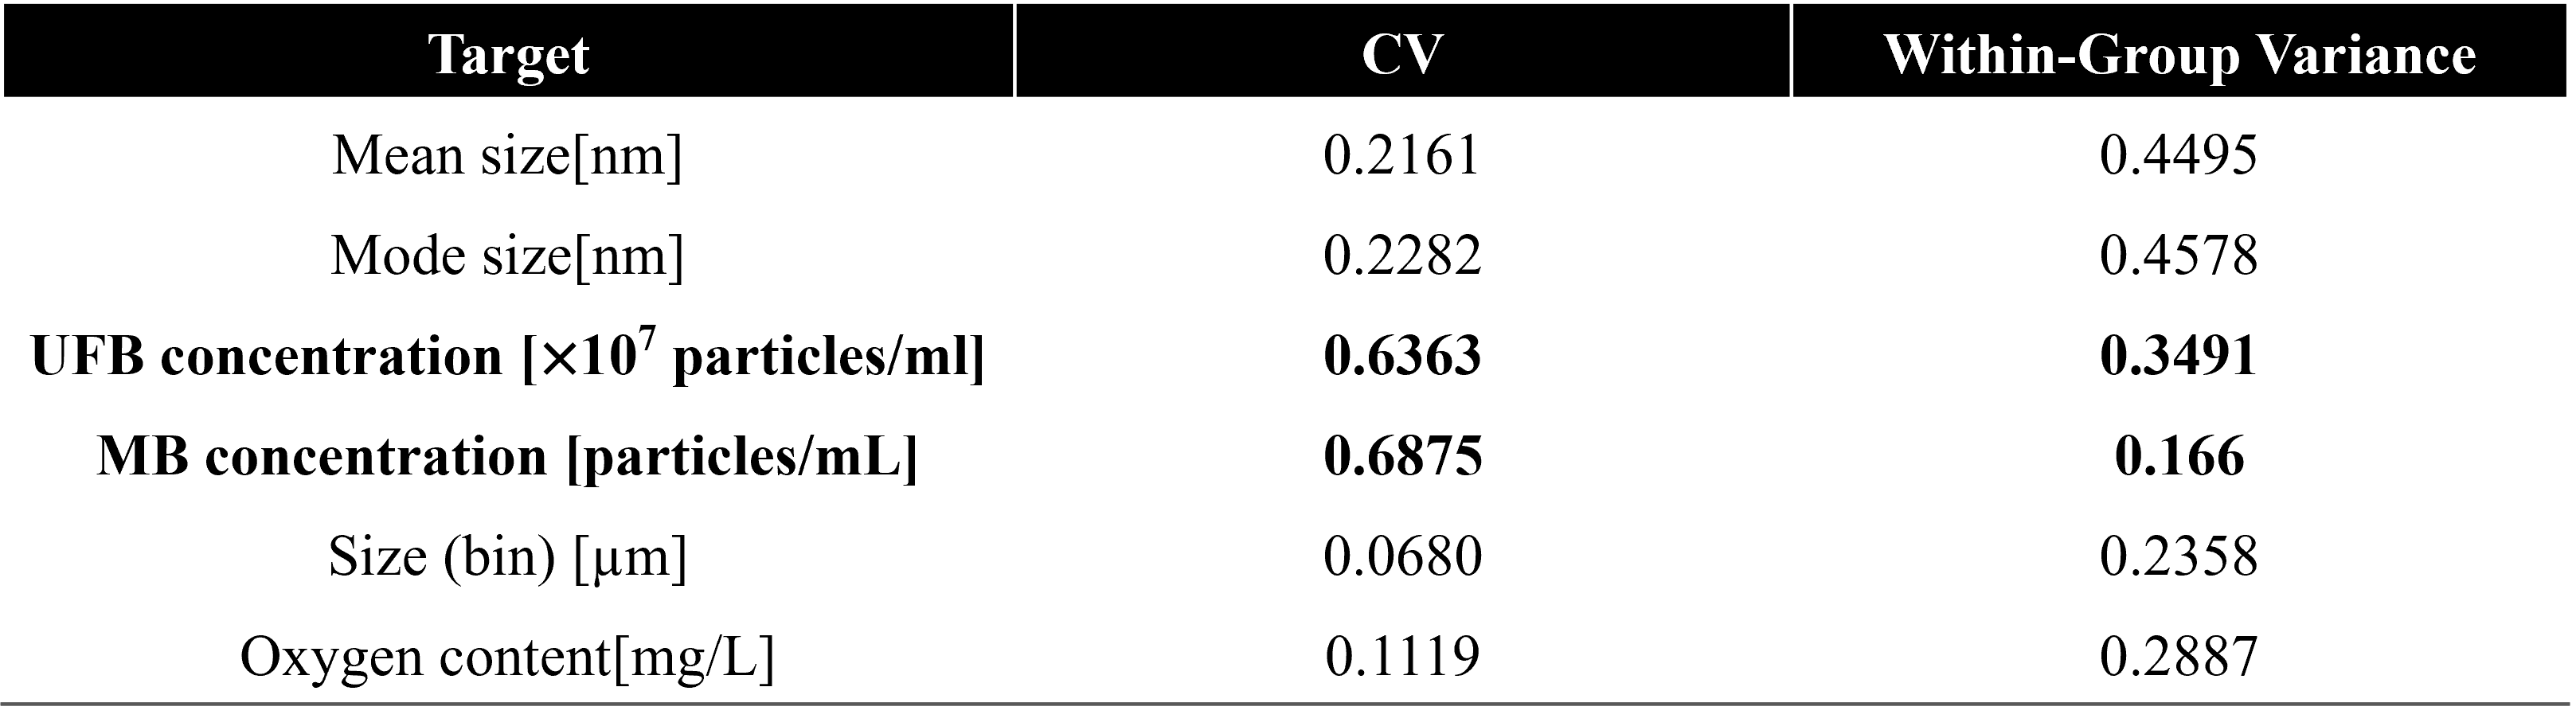
\includegraphics[width=\linewidth]{figures/table1_coefficient_of_variation_and_within_group_variance.png}
    \label{tab_cv}
\end{table}

選定した 3 つの目的変数と 6 つの説明変数について，各説明変数と目的変数の線形な関係の強さを把握するため，Pearson の積率相関係数を式(\ref{eq_pearson})により算出した．

\begin{equation}
    r_{e,t} = \frac{ \sum_{i=1}^{N} (x_i^e - \bar{x}^e)(y_i^t - \bar{y}^t) }{ \sqrt{ \sum_{i=1}^{N} (x_i^e - \bar{x}^e)^2 } \sqrt{ \sum_{i=1}^{N} (y_i^t - \bar{y}^t)^2 } }
    \label{eq_pearson}
\end{equation}

\noindent
ここで $ e $ は説明変数の種類，$ t $ は目的変数の種類，$ x_i^e $ は説明変数 $ e $ の $ i $ 番目のサンプルにおける値，$ y_i^t $ は目的変数 $ t $ の $ i $ 番目のサンプルにおける値，$ \bar{x}^e $，$ \bar{y}^t $ はそれぞれの平均，$ N $ はサンプル数である．
$ r_{e,t} $ は説明変数 $ e $ と目的変数 $ t $ の間の相関係数であり，$ -1 $ から $ 1 $ の値を取り，絶対値が大きいほど両変数間の線形な関係が強いことを示す．
なお，説明変数同士および目的変数同士の相関は本研究の関心対象外であるため算出していない．
図\ref{fig_correlation}に，算出した相関係数を示す．
Discharge tube は MB 濃度と負の相関（$ r = -0.46 $），酸素含量と正の相関（$ r = 0.65 $）を示し，操作条件の中で最も目的変数との関連が強い．
また，UFB 濃度は Flow speed (oxygen)（$ r = 0.38 $），Water volume（$ r = -0.40 $）とそれぞれ中程度の相関を示し，単一の説明変数に支配されない傾向がみられる．
このように，操作条件と目的変数の間に一定の線形相関が存在することから，操作条件から目的変数を予測する機械学習モデルの構築が有効であると考えられる．

\begin{figure}[H]
    \centering
    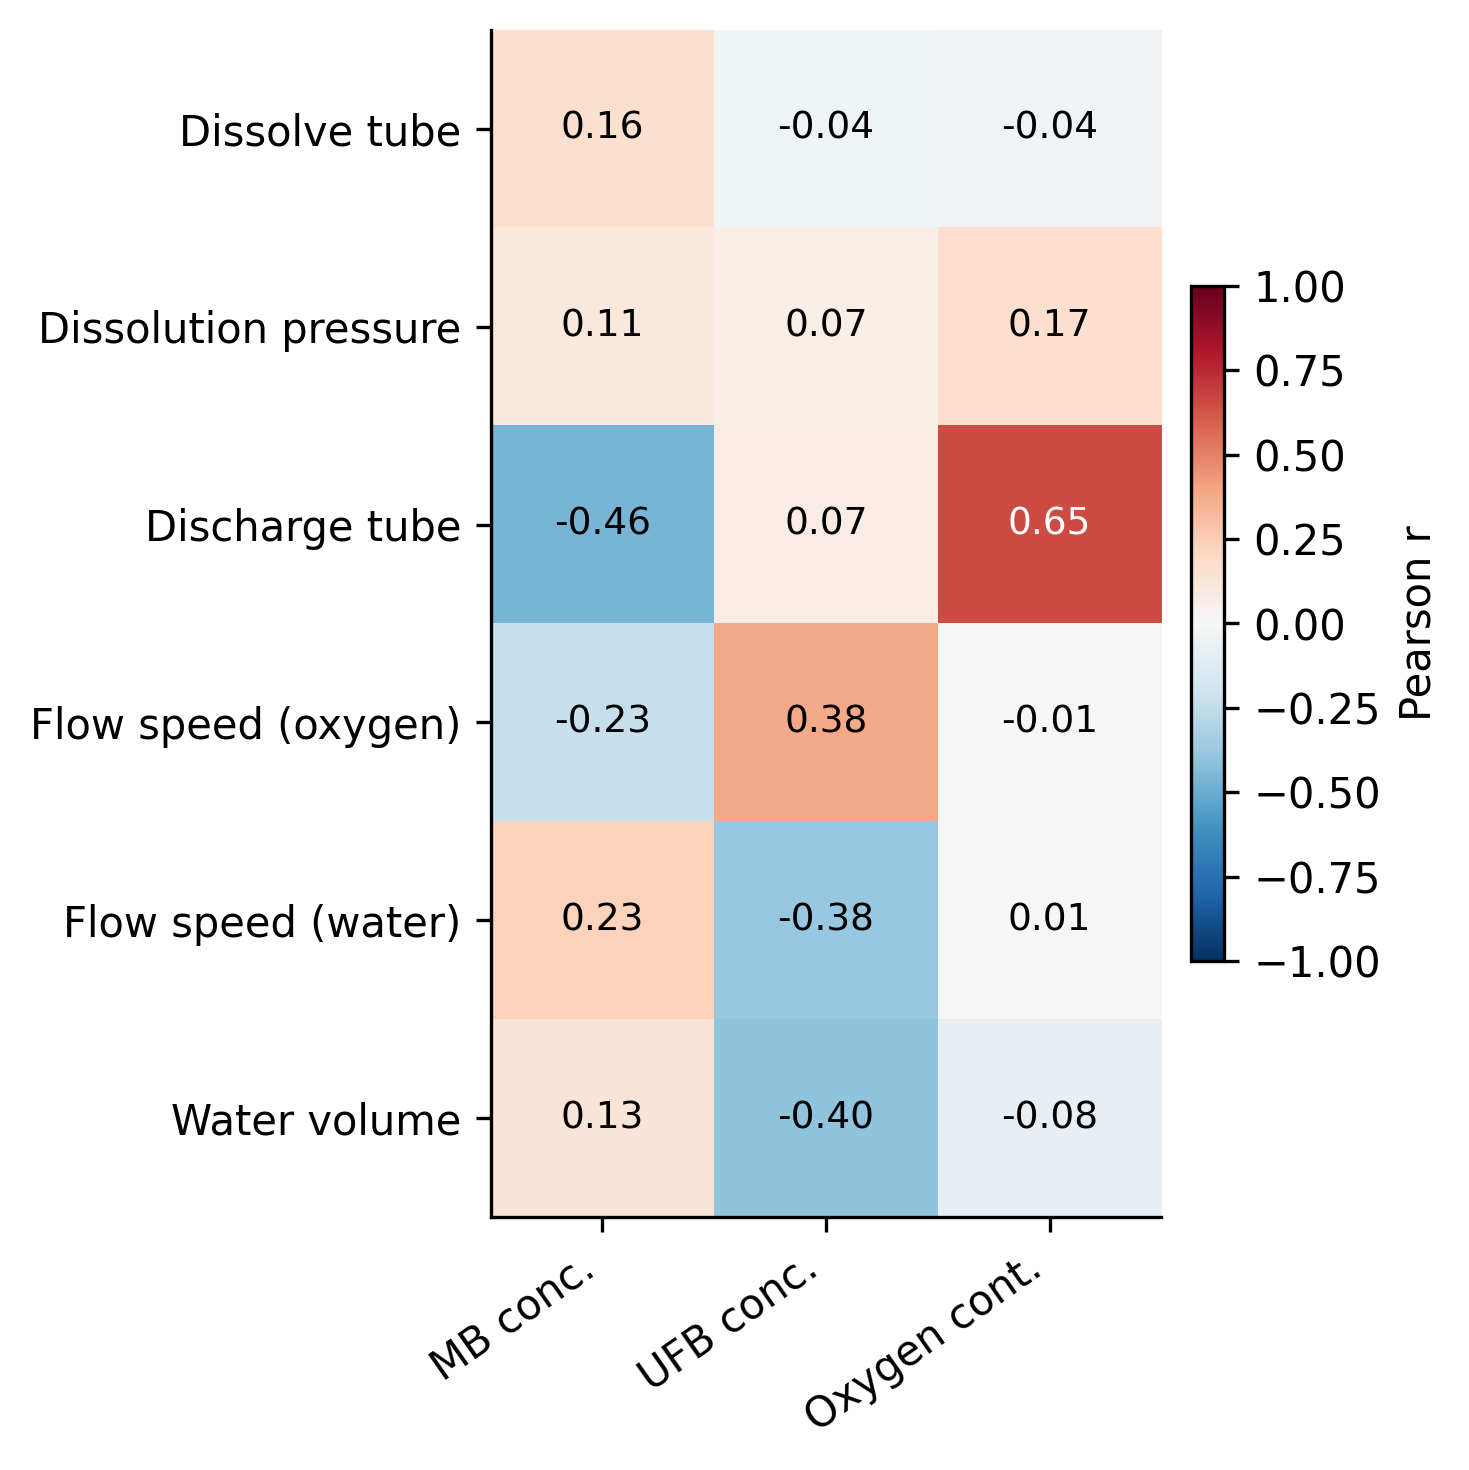
\includegraphics[width=\linewidth]{figures/figure2_correlation_coefficient.png}
    \caption{説明変数と目的変数の相関係数}
    \label{fig_correlation}
\end{figure}
